\section{Literature Review}
\label{sec:review}
%

\subsection{Introduction}
\subsubsection{Overview of the existing fluids hydraulic test rig}

\begin{figure}[ht]
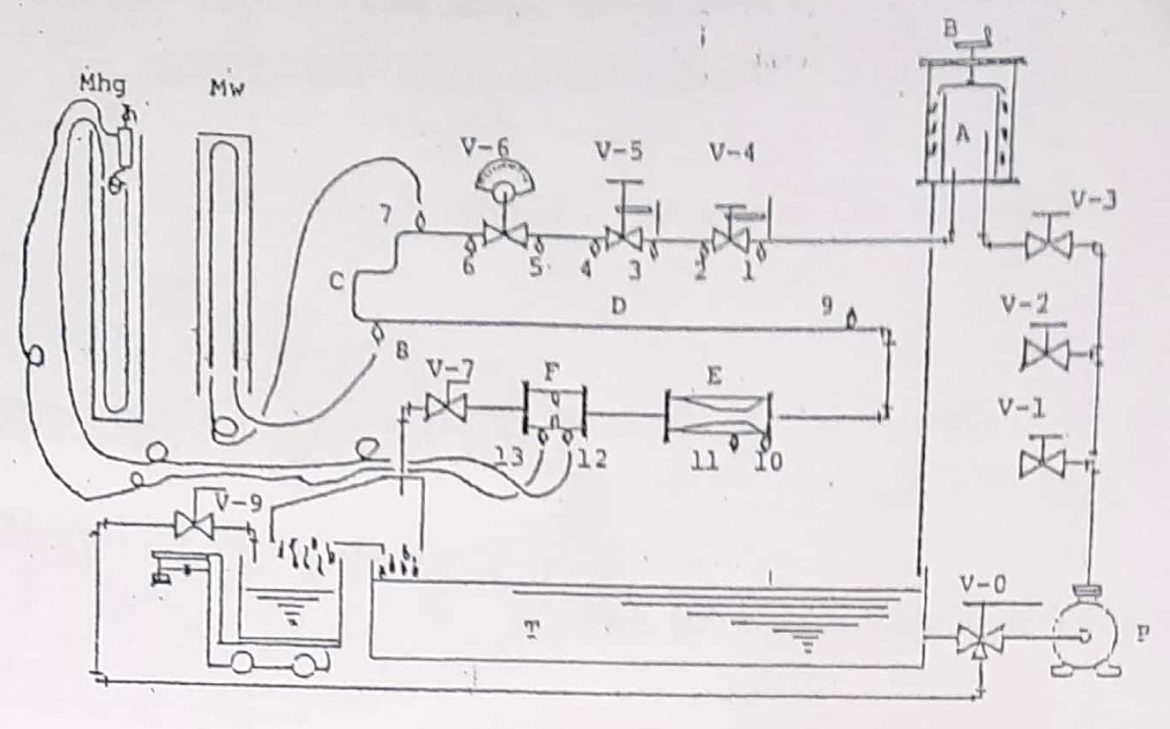
\includegraphics[width=0.9\linewidth]{Figures/syntheticHydroexperimentalMachine.png}
\centering
\caption{Fluids Hydraulic Test Rig }
\label{fig:fluid_hydraulic_test_rig}
\end{figure}

\begin{table}[ht]
  \begin{center}
    \leavevmode
     \begin{tabular}{|c | p{0.7\linewidth}|}\hline
     Part Number & Description \\ \hline
      1-13 & Pressure taps \\
      \hline
      V-1,2,3 & Sluice Valve \\
      \hline
      V-0 & Three direction valve \\
      \hline
      V-4 & Sluice valve (\ac{WD}21\ac{P} model 1-in, 32P and 33F model 1.25 in) \\
      \hline
      V-5 & Glove valve (WD21P model 1-in, 32P and 33F model 1.25 in) \\
      \hline
      V-6,7 & Cock (WD21P model 1-in, 32P and 33F model 1.25 in) \\ 
      \hline
      A & Overflow tank \\ 
      \hline
      B & Handle for applying pressure \\ 
      \hline
      C & Elbow section (WD21P model 1-in, 32P and 33F model 1.25 in) \\ 
      \hline
      D & Straight Pipe Section (WD21P model 1-in, 1m long, 32P and 33F model 1.25 in) \\ 
      \hline
      E & Venturi-meter, (WD21P model 1-in, 32P and 33F model 1.25 in) \\ 
      \hline
      F & Orifice meter, (WD21P model 1-in, 32P and 33F model 1.25 in). \\ 
      \hline
      Mhg & Mercury manometer. \\ 
      \hline
      Mw & Water manometer. \\ 
      \hline
      P & Volute Pump. \\ 
      \hline
      T & Main tank. \\ 
      \hline
    \end{tabular}
    \hangcaption{List of parts in the existing fluids hydraulics test rig}
    \label{table:1}
  \end{center}
\end{table}

The Fluids Hydraulic Test Rig shown in figure \ref{fig:fluid_hydraulic_test_rig} consists of a water loop system, two flow measuring devices, the venturi, and the orifice meter connected in series with pressure taps across each device connected to vertical differential manometers located at the front end of the machine. The flow rate is controlled by a gate valve located at the discharge side of the machine. A diverter at the end of the machine directs the discharge from the apparatus into a collecting trough where it is measured and then pumped back into the reservoir.   

\subsection{Venturi}

A venturi meter is a flow measuring device used to measure the properties of a flowing fluid. It can also be used to increase the velocity of a flowing fluid at a particular point in a pipe. It works on the principle of Bernoulli’s Theorem\cite{pockman1940bernoulli}. A venturi meter causes a change in the fluid pressure and velocity properties\cite{hutagalung2019estimation}. A high-pressure, low-velocity fluid flowing through a venturi suddenly assumes low-pressure, high-velocity.

\subsubsection{Construction}

\begin{figure}[ht]
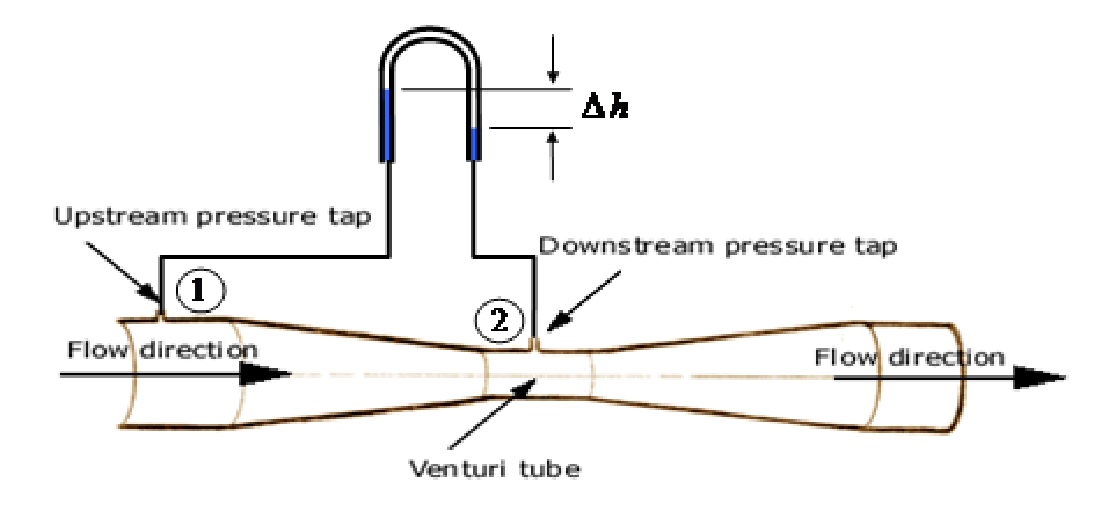
\includegraphics[width=0.9\linewidth]{Figures/venturi.png}
\centering
\caption{Venturi meter}
\label{fig:venturi}
\end{figure}

The construction of a venturi meter is shown in figure \ref{fig:venturi}. It has a constriction within itself.

\subsubsection{Coefficient of discharge derivation}

The pressure difference between the upstream and the downstream flow, ∆h, can be expressed as a function of the flow rate.
\par
Assuming an incompressible flow and no frictional losses, the Bernoulli’s equation can be applied to points 1 and 2 of the venturi meter as shown in equation \ref{eq:1} 

\begin{equation}
\label{eq:1}
\frac{P_{1}}{\gamma}+\frac{V_{1}^{2}}{2 g}+Z_{1}=\frac{P_{2}}{\gamma}+\frac{V_{2}^{2}}{2 g}+Z_{2}
\end{equation}

Using the continuity equation \ref{eq:2} 

\begin{equation}
\label{eq:2}
\mathrm{Q}=\mathrm{A}_{1} \mathrm{~V}_{1}=\mathrm{A}_{2} \mathrm{~V}_{2}
\end{equation}

Equation \ref{eq:1} becomes

\begin{equation}
\label{eq:3}
\frac{P_{1}-P_{2}}{\gamma}+Z_{1}-Z_{2}=\frac{V_{2}^{2}}{2 g}\left[1-\left(\frac{A_{2}}{A_{1}}\right)^{2}\right]
\end{equation}

\begin{equation}
\label{eq:4}
V_{2}=\frac{1}{\sqrt{1-\left(\frac{A_{2}}{A_{1}}\right)^{2}}} \sqrt{2 g\left(\frac{P-P_{2}}{\gamma}+\left(Z_{1}-Z_{2}\right)\right)}
\end{equation}

Theoretical discharge, $Q_{theo}$ is given by equation \ref{eq:5}
\begin{equation}
\label{eq:5}
Q_{\text {theo }}=A_{2} V_{2}=\frac{A_{2}}{\sqrt{1-\left(\frac{A_{2}}{A_{1}}\right)^{2}}} \sqrt{2 g\left(\frac{P_{1}-P_{2}}{\gamma}+\left(Z_{1}-Z_{2}\right)\right)}
\end{equation}

The term
\begin{equation}
\frac{P_{1}-P_{2}}{\gamma}+\left(Z_{1}-Z_{2}\right)
\end{equation}
 represents the difference in the piezometric head (∆h) between the two sections 1 and 2. The above expression for $V_{2}$ is obtained based on the assumption of one-dimensional frictionless flow. Hence the theoretical flow can be expressed as in equation \ref{eq:6}
 \begin{equation}
 \label{eq:6}
Q_{\text {theo }}=A_{2} V_{2}=\frac{A_{2}}{\sqrt{1-\left(\frac{A_{2}}{A_{1}}\right)^{2}}} \sqrt{2 g(\Delta h)}
\end{equation}
Thus
\begin{equation}
\label{eq:7}
Q_{\text {theo }}=\sqrt{\frac{2 g \Delta h}{\left(\frac{.1}{A_{2}^{2}}-\frac{1}{A_{1}^{2}}\right)}}
\end{equation}
From the above assumptions, the actual flow rate $Q_{act}$ differs from $Q_{theo}$ and the ratio between them is called the discharge coefficient, $C_{d}$ which can be expressed as in  equation \ref{eq:8}
\begin{equation}
\label{eq:8}
C_{d}=\frac{Q_{a c t}}{Q_{\text {theo }}}
\end{equation}

\subsubsection{Construction Standards}
The value of $C_{d}$ differs from one flowmeter to the other depending on the flowmeter geometry and Reynold’s number. The discharge coefficient is always less than 1 due to various losses such as friction losses, and area contraction
\begin{figure}[ht]
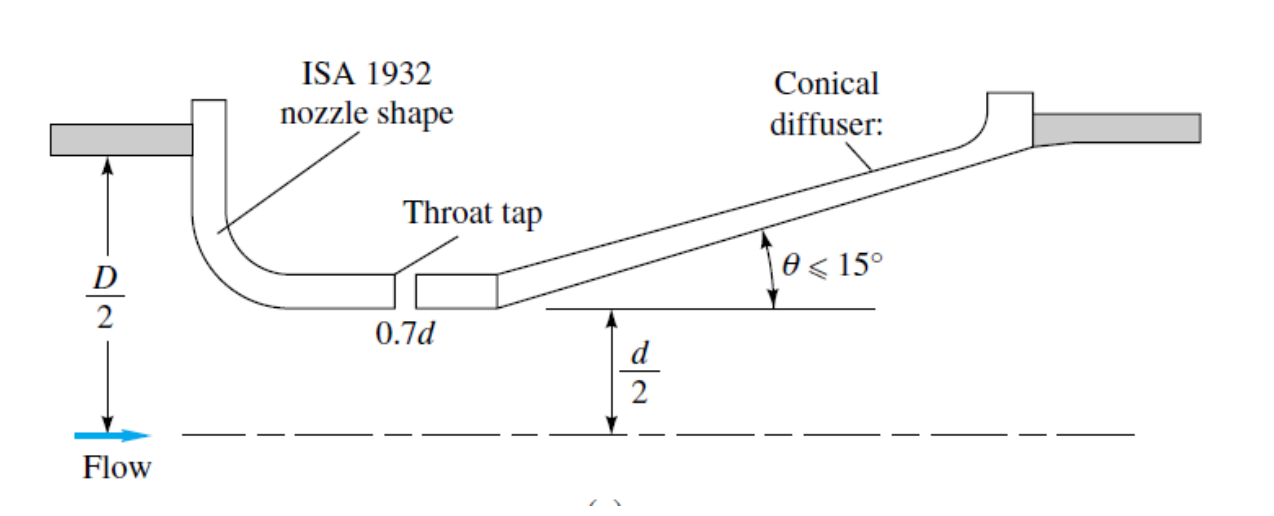
\includegraphics[width=0.9\linewidth]{Figures/standard.png}
\centering
\caption{ International Standard Shapes for Venturi Nozzle }
\label{fig:International_Standard_Shapes_for_Venturi_Nozzle}
\end{figure}
The modern venturi nozzle above consists of an ISA 1932 nozzle entrance and a conical expansion of half-angle no greater than $15^0$ \cite{thorn201720}. It is intended to be operated in a narrow Reynolds number range of 1.5x$10^6$ to 2x$10^6$ \cite{salomo2019estimation}. The coefficient of discharge is 0.95 – 0.98 for a venturi meter \cite{stauffer2019multiple}.

\subsection{Orifice Meter}
An orifice consists of a flat plate that has a sharp-edged hole accurately machined in it and placed concentrically in a pipe as shown in figure \ref{fig:orifice_with_flow} \cite{pereira2009flow}. As the fluid flows through the pipe, the flow suddenly contracts as it approaches the orifice and then suddenly expands after the orifice back to the full pipe diameter. This forms a vena contracta or a throat immediately past the orifice. This reduction in flow pattern at the vena contracta causes increased velocity and hence lower pressure at the throat as shown in figure \ref{fig:Vena_Contracta} \cite{shah2012analysis}.

\begin{figure}[ht]
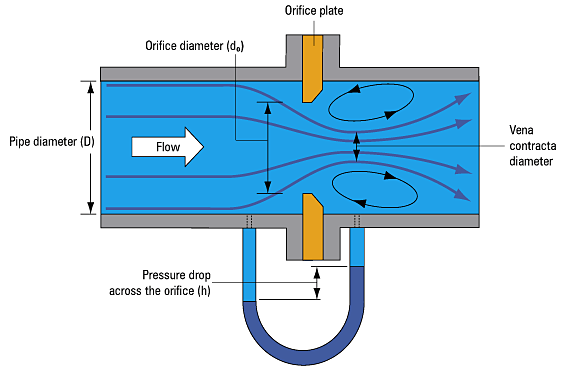
\includegraphics[width=0.9\linewidth]{Figures/orifice_with_flow.png}
\centering
\caption{Orifice Meter}
\label{fig:orifice_with_flow}
\end{figure}

The pressure difference between the inlet, with the full flow and the outlet at the throat, can then be used to measure the liquid flow rate. Because of the sudden contraction at the orifice and the subsequent sudden expansion after the orifice, the coefficient of discharge $C_{d}$ for the orifice meter is much lower than that of a venturi meter \cite{reader2015orifice}.

\begin{figure}[ht]
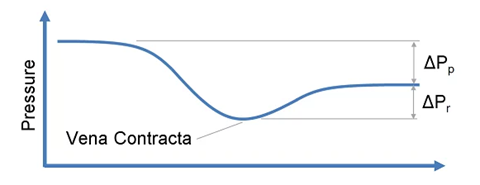
\includegraphics[width=0.9\linewidth]{Figures/venaContracta.png}
\centering
\caption{ Vena Contracta }
\label{fig:Vena_Contracta}
\end{figure}

Figure \ref{fig:Vena_Contracta} above shows the graphical trend of pressure variation across the orifice plate. It can be seen that at the contracted section, the pressure magnitude is the least after which the pressure head is restored but to decremented value in comparison to the pressure at the inlet. This is because of frictional losses incurred as the fluid traverses the pipe length \cite{shah2012analysis}.

\subsubsection{Coefficient of discharge derivation}

The orifice outflow velocity can be calculated by applying Bernoulli’s equation (for a steady, incompressible, frictionless flow) to a large reservoir with an opening (orifice) on its side \cite{morrison1990flow}.

\begin{equation}
\label{eq:9}
v_{i}=\sqrt{2 g h}
\end{equation}

where h is the height of fluid above the orifice. This is the ideal velocity since the effect of fluid viscosity is not considered in deriving the above equation. The actual flow velocity, however, is smaller than vi and is calculated as

\begin{equation}
\label{eq:10}
v=C_{v} \sqrt{2 g h}
\end{equation}

$C_{v}$ is the coefficient of velocity, which allows for the effects of viscosity; therefore, $C_{v}$ <1. The actual outflow velocity calculated by the above equation is the velocity at the vena contracta, where the diameter of the jet is the least and the flow velocity is at its maximum.

The actual outflow rate may be calculated as:
\begin{equation}
\label{eq:11}
Q=v A_{c}
\end{equation}

where $A_{c}$ is the flow area at the vena contracta. $A_{c}$ is smaller than the orifice area, $A_{0}$, and is given by:
\begin{equation}
\label{eq:12}
A_{c}=C_{c} A_{o}
\end{equation}

where $C_{c}$ is the coefficient of contraction; therefore, $C_{c}$ < 1.

Substituting v and $A_{c}$ from equation \ref{eq:10} and equation \ref{eq:12} into equation \ref{eq:11} results in:
\begin{equation}
\label{eq:13}
Q=C_{v} C_{c} A_{0} \sqrt{2 g h}
\end{equation}
The product of $C_{c}$ x $C_{v}$  is called the coefficient of discharge $C_{d}$. Therefore:
\begin{equation}
\label{eq:14}
Q=C_{d} A_{0} \sqrt{2 g h}
\end{equation}

\subsection{Discharge Collection}

\begin{figure}[ht]
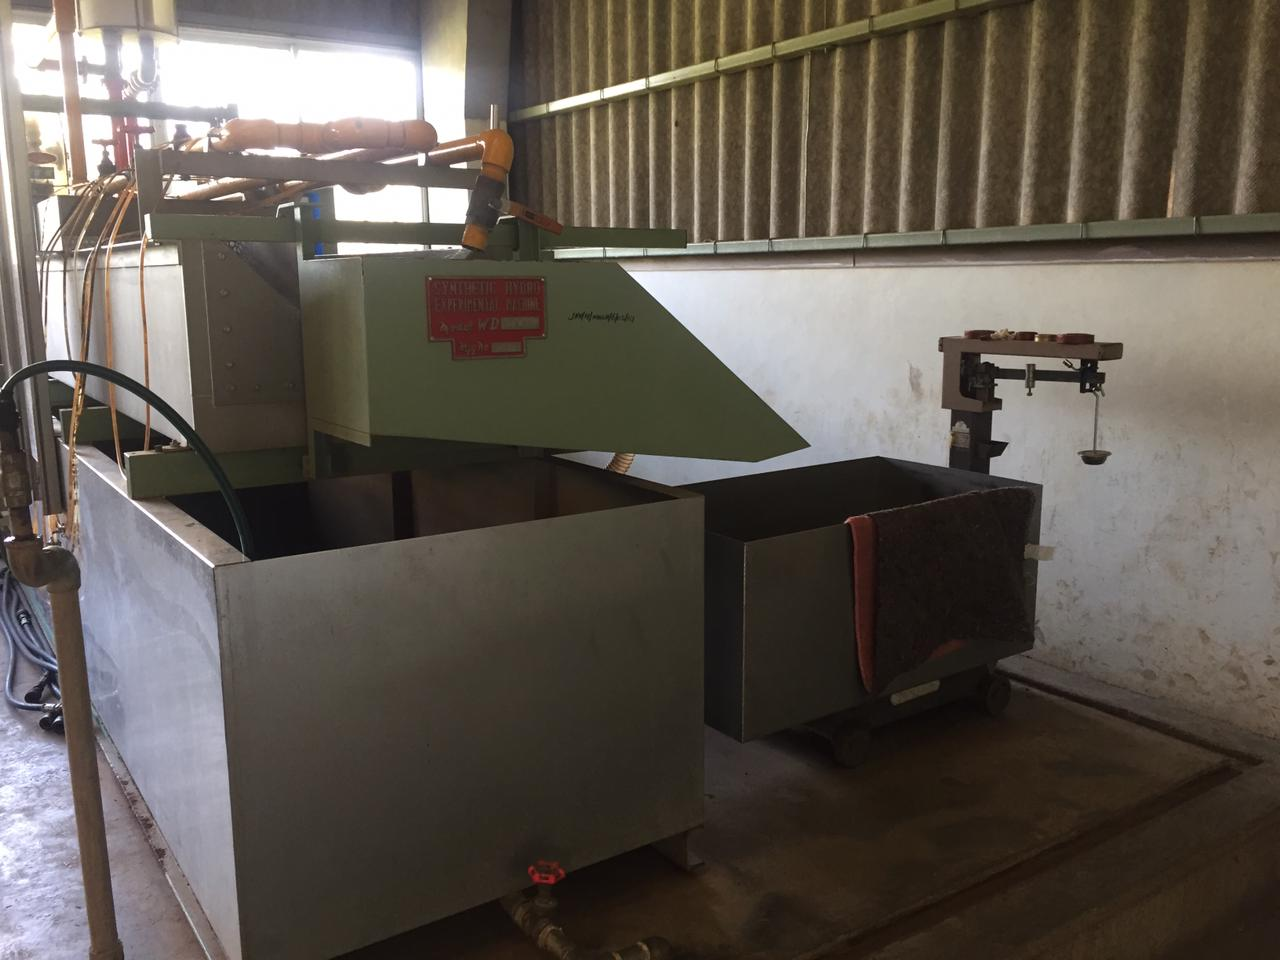
\includegraphics[width=0.9\linewidth]{Figures/discharge.jpeg}
\centering
\caption{Discharge Collection Construction}
\label{fig:Discharge_Collection_Construction}
\end{figure}

Figure \ref{fig:Discharge_Collection_Construction} shows the construction of the discharge collection unit. The trough is used to divert the discharge to a collection tank for weight measurement.

\par

During the experiment to establish a relationship between the coefficient of discharge of both the Venturi and the Orifice, and the difference in pressure, this unit is used to collect the discharge. It is slid in, when the timer starts, below the discharge valve to collect the discharge, and slid out when the timer stops. It is a huge piece of metal bent to a funnel-like shape to divert the discharge to a collecting trough for weight measurement.

\subsection{Gap Analysis}
Synchronizing time and temperature measurement with discharge collection proves to be difficult with this machine since the discharge collection mechanism is wholly mechanical. The flow rate is controlled by a gate valve in small steps which is determined by human intuition and can be inconsistent. In addition, weight measurement of the discharge uses calibrated weights whose resolution is too wide. These limitations often results in processed values outside the tolerable range.  

